%*****************************************************************
\subsection{Calibration Results}\label{sub:bc_calibration_results}
%*****************************************************************

\clearpage
\begin{sidewaysfigure}
	\centering
	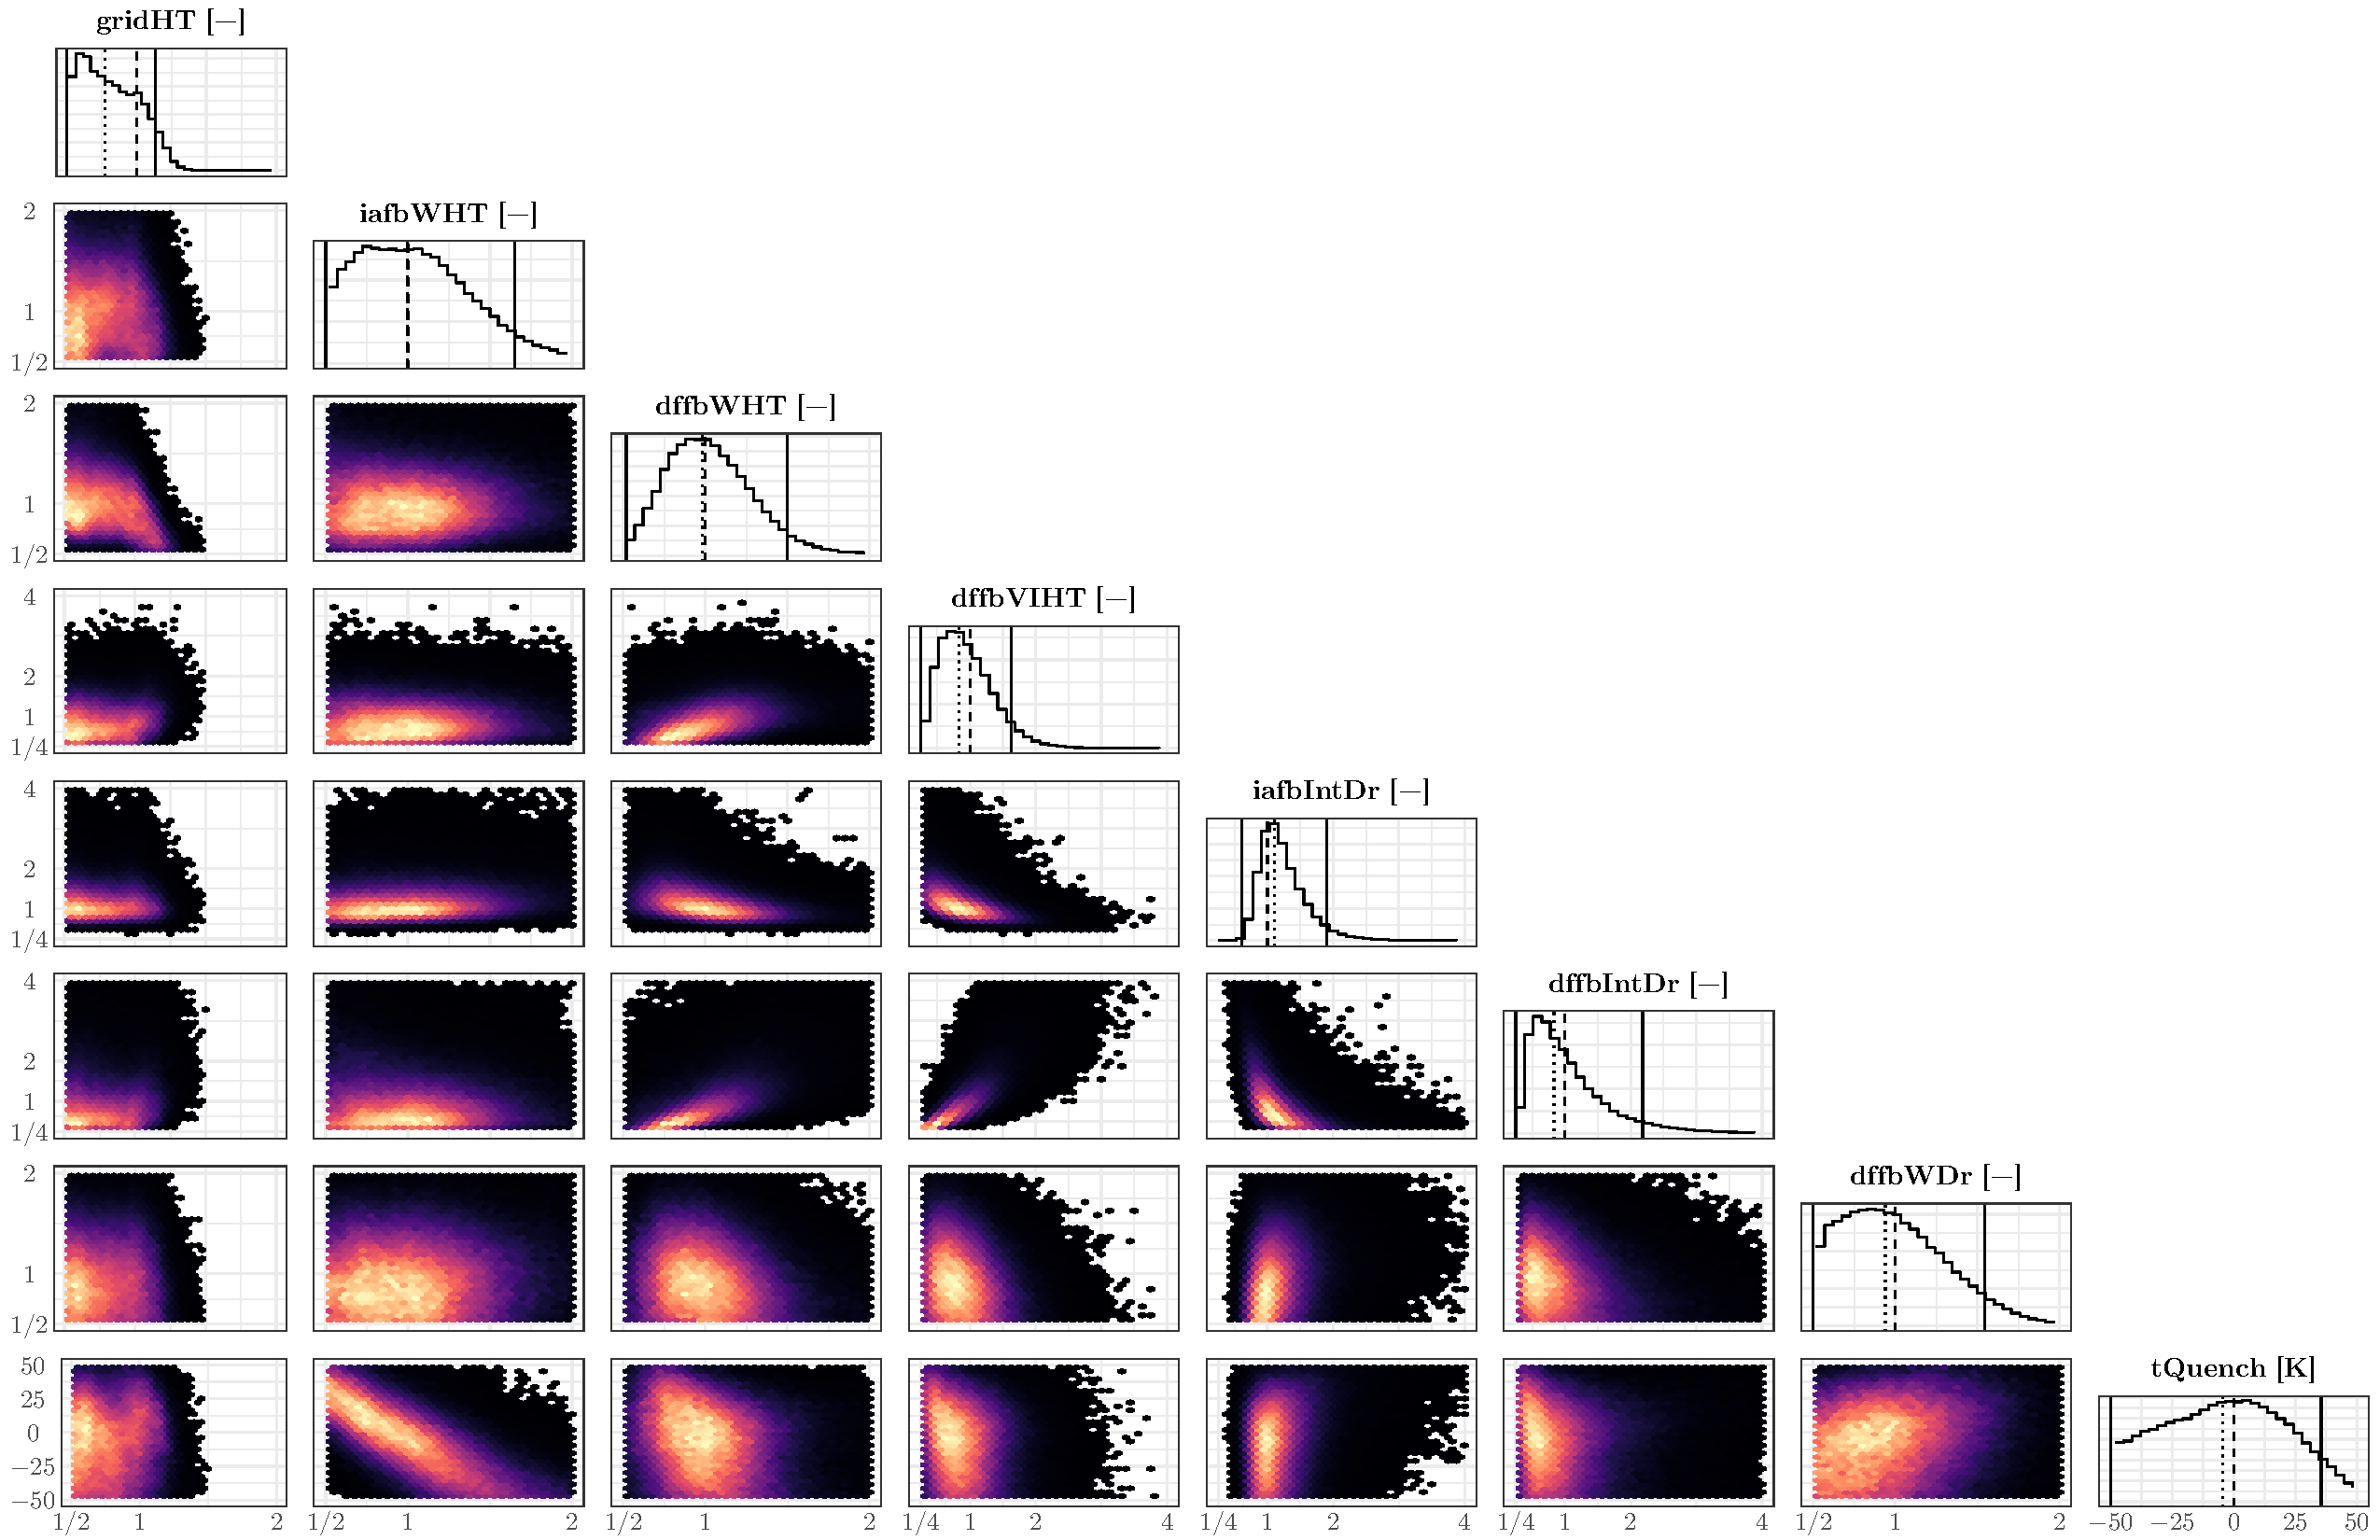
\includegraphics[width=0.90\textwidth]{../figures/chapter5/figures/plotEnsAllDiscCentered}
		\captionof{figure}[Univariate and bivariate marginals of the posterior samples for each of the $8$ model parameters. Calibration with model bias term.]{Univariate and bivariate marginals of the posterior samples for each of the $8$ model parameters. Solid lines, dashed, and dotted lines indicate the \glspl[hyper=false]{hpdi}, the nominal parameter values, and the posterior median parameter values. Calibration with model bias term.}
	\label{fig:ch5_plot_ens_all_disc_centered}
\end{sidewaysfigure}
\clearpage

\glspl[hyper=false]{hpdi}

\clearpage
\begin{sidewaystable}
\caption{Summary of calibration results. The three numbers in brackets are the lower $95\%$\gls[hyper=false]{hpdi}, the median, and the $95\%$ upper \gls[hyper=false]{hpdi}, respectively for the prior and all the posteriors.}
\label{tab:trace_model_parameter_1}
\centering
\newcolumntype{Y}{>{\RaggedRight\arraybackslash}X}
\begin{tabularx}{1.025\textwidth}{@{}ccccccccc@{}}
\toprule
\multirow{2}{*}{No.} & \multirow{2}{*}{Parameter} & \multirow{2}{*}{Prior} &    \multicolumn{6}{c}{Posterior Summaries (lower HPDI, median, upper HPDI)} \\
                                           \cmidrule{4-9}
 &  ID                &   Summaries     & \footnotesize{w/ Bias} &  \footnotesize{w/ Bias, TC Only} &  \footnotesize{w/ Bias, DP Only} & \footnotesize{w/ Bias, CO Only} & \footnotesize{w/ Bias, excl. \texttt{dffbVIHTC}} & \footnotesize{w/o Bias}\\ \midrule
\footnotesize{$1$} & \texttt{gridHT}   &\footnotesize{$[0.50, 1.00,2.00]$}&\footnotesize{$[0.50,0.77,1.14]$} &\footnotesize{$[0.50,0.78,1.21]$}   &\footnotesize{$[0.50,0.92,1.70]$}  &\footnotesize{$[0.50,0.95,1.82]$}  &\footnotesize{$[0.50,0.80,1.14]$}  &\footnotesize{$[0.50,0.94,1.05]$}\\
\footnotesize{$2$} &\texttt{iafbWHT}   &\footnotesize{$[0.50, 1.00,2.00]$}&\footnotesize{$[0.50,1.00,1.65]$} &\footnotesize{$[0.50,0.92,1.71]$}   &\footnotesize{$[0.50,1.06,1.85]$}  &\footnotesize{$[0.50,0.97,1.84]$}  &\footnotesize{$[0.50,1.02,1.66]$}  &\footnotesize{$[0.50,0.52,1.99]$}\\
\footnotesize{$3$} &\texttt{dffbWHT}   &\footnotesize{$[0.50, 1.00,2.00]$}&\footnotesize{$[0.52,0.98,1.50]$} &\footnotesize{$[0.50,0.97,1.56]$}   &\footnotesize{$[0.50,0.85,1.77]$}  &\footnotesize{$[0.50,0.95,1.85]$}  &\footnotesize{$[0.57,1.06,1.57]$}  &\footnotesize{$[0.50,0.52,0.66]$}\\
\footnotesize{$4$} &\texttt{dffbVIHT}  &\footnotesize{$[0.25, 1.00,4.00]$}&\footnotesize{$[0.25,0.83,1.63]$} &\footnotesize{$[0.25,0.90,1.89]$}   &\footnotesize{$[0.25,0.92,2.98]$}  &\footnotesize{$[0.25,0.75,2.63]$}  &\footnotesize{$[0.25,1.00,4.00]$}  &\footnotesize{$[3.50,3.90,4.00]$}\\
\footnotesize{$5$} &\texttt{iafbIntDr} &\footnotesize{$[0.25, 1.00,4.00]$}&\footnotesize{$[0.61,1.10,1.90]$} &\footnotesize{$[0.25,1.27,3.50]$}   &\footnotesize{$[0.48,1.11,2.62]$}  &\footnotesize{$[0.25,1.03,3.48]$}  &\footnotesize{$[0.65,1.02,1.63]$}  &\footnotesize{$[0.45,0.57,0.69]$}\\
\footnotesize{$6$} &\texttt{dffIntDr}  &\footnotesize{$[0.25, 1.00,4.00]$}&\footnotesize{$[0.25,0.83,2.18]$} &\footnotesize{$[0.25,0.97,2.90]$}   &\footnotesize{$[0.25,1.17,3.32]$}  &\footnotesize{$[0.25,1.22,3.51]$}  &\footnotesize{$[0.49,1.03,1.80]$}  &\footnotesize{$[0.31,0.96,1.88]$}\\
\footnotesize{$7$} &\texttt{dffbWDr}   &\footnotesize{$[0.50, 1.00,2.00]$}&\footnotesize{$[0.50,0.94,1.55]$} &\footnotesize{$[0.50,1.01,1.87]$}   &\footnotesize{$[0.50,0.97,1.60]$}  &\footnotesize{$[0.50,1.01,1.87]$}  &\footnotesize{$[0.50,0.92,1.51]$}  &\footnotesize{$[0.50,0.52,0.60]$}\\
\footnotesize{$8$} &\texttt{tQuench}   &\footnotesize{$[-50.0,0.00,50.0]$}&\footnotesize{$[-50.,-4.6,35.4]$} &\footnotesize{$[-50.0,-7.9,36.9]$}  &\footnotesize{$[-50.0,-3.5,40.3]$} &\footnotesize{$[-49.8,-1.9,44.6]$} &\footnotesize{$[-50.0,-7.7,30.9]$} &\footnotesize{$[-49.5,48.4,50.0]$}\\ 
\bottomrule
\end{tabularx}
\end{sidewaystable}
\clearpage
